\section{Socorro Modular structure}

What follows will be a description of the current Socorro code
structure as well as a description of more specific tricks and
techniques we have employed in the code.  Let the reader be warned
that the Socorro code is in a perpetual state of development, and
that this section is meant to give enough of a framework
to the reader so that he/she can look over any module in Socorro
with some idea as to its purpose.

While the debate rages on between the use of global versus local
variables in the FORTRAN community, Socorro encapsulates almost all
program state into a single variable of \verb+type(config_obj)+ (the
various runtime support functions are the only exception to this).
The initialization of a variable of \verb+type(config_obj)+
is the entire self-consistent calculation.

The \verb+type(config_obj)+, its constituent types and the rest of
their descendants can be rendered in a graph shown in figure
\ref{datafig}.  Each module in the diagram is responsible for
maintaining its own rep-invariants.  If the \verb+config_mod+
module defines a function which modifies the \verb+type(external_obj)+
of variable of \verb+type(config_obj)+, that function must also
restore the self-consistency of the \verb+type(config_obj)+ variable
as that is one of the rep-invariant of \verb+type(config_obj)+.

The universal application of this principle drives all computation
in Socorro, currently.  All mutable types in Socorro
come with an \verb+update()+ subroutine, which allows them to
modify their constituents and perform whatever necessary computations
must be done to restore the rep-invariants (see figure \ref{modifyfig}).
One technique we are using to implement this efficiently is
discussed in section \ref{ghostsec}.

\begin{figure}
\begin{center}
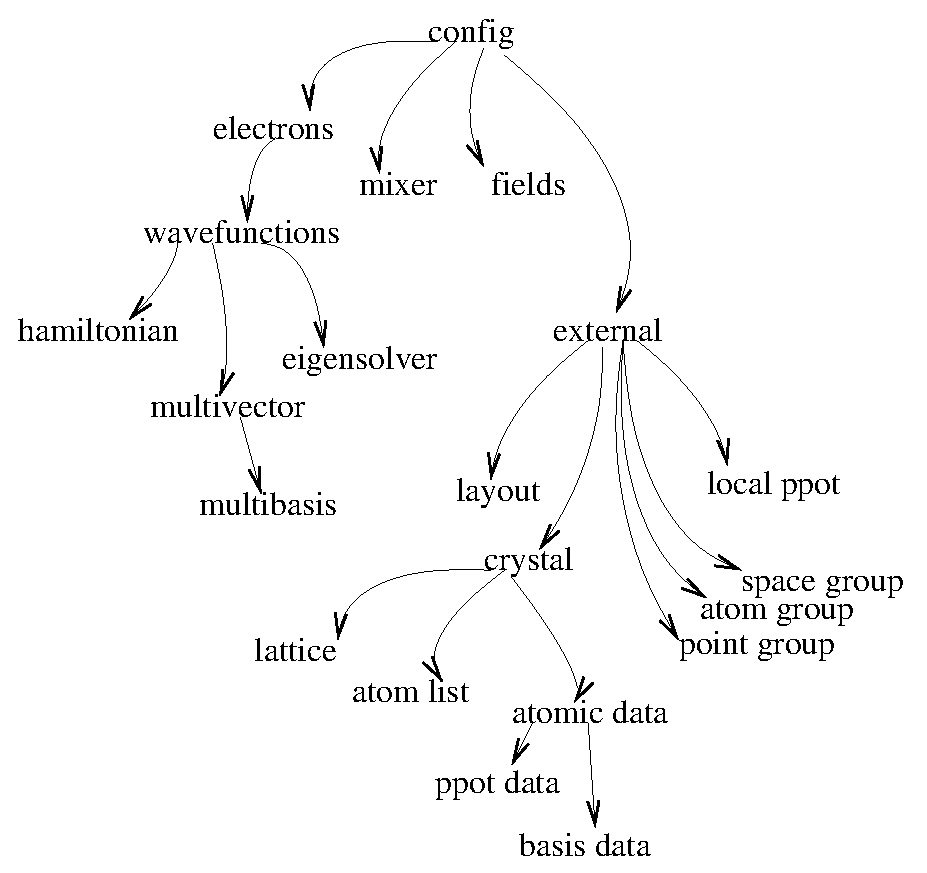
\epsfig{file=figs/datamap.eps}
\caption{A map of the data hierarchy in Socorro}
\label{datafig}
\end{center}
\end{figure}

\begin{figure}
\begin{center}
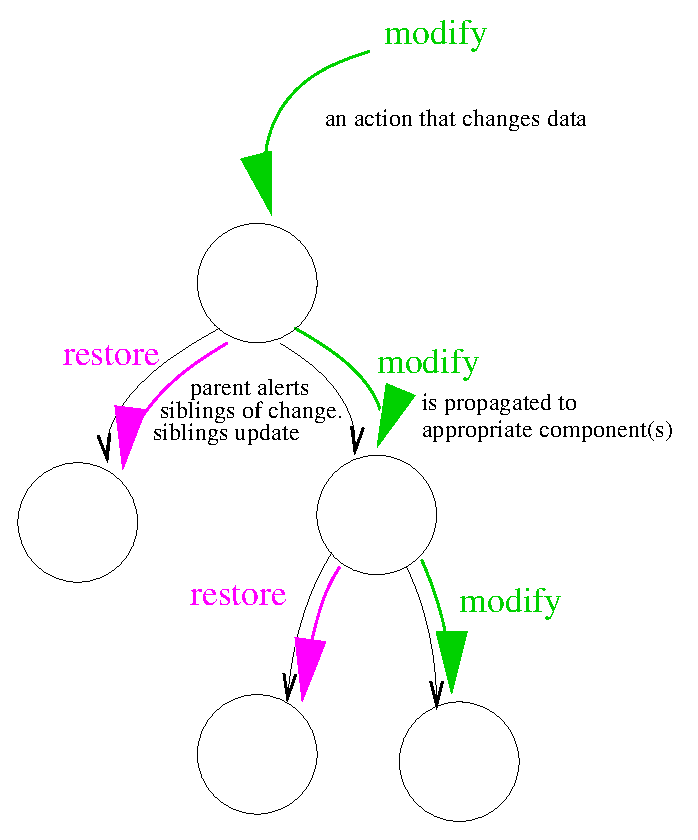
\epsfig{file=figs/constraint.eps}
\caption{Iterative dynamics are driven by the preservation of representation
invariants.}
\label{modifyfig}
\end{center}
\end{figure}

\subsection{Documentation}

People who program do not like to document what they write.
This is a sociological fact.  The person who writes a program,
when he/she does document, will tend to forgive the brevity
or opaqueness of his commentary.  This is a psychological fact.
In light of these two facts, it is best to adopt a documentation
process which minimizes effort in both creation and modification
of program documentation.

The free form Socorro files place procedure comments in the
procedure headers and allow the implementer the option of exporting
arbitrary code into the documentation for that module, to spare
him/her the tiresome task of recasting the same information into
the documentation.  Exporting code to documentation
prevents the documentation and code
from drifting apart.  Note: the fixed form Socorro files (which
will eventually be converted to free form) follow
an earlier convention which was abandoned primarily because
it promoted code/doc drift.

Documented blocks of code start with a line which begins with the
string \verb+!doc$+ in the program text.  If anything else is on that
line, it is stripped of the \verb+!doc$+, capitalized, and exported.
All subsequent lines are exported (stripping out leading \verb+!+
symbols), until the next occurrence of a \verb+!cod$+ which terminates
the documentation block.

For example, the following module header,
\begin{verbatim}
!doc$
      MODULE LATTICE_MOD

!     The lattice module hold basic lattice concepts: the lattice vectors
!     the lattice reciprocal vectors.

      use kind_mod
      use core_mod
      use diary_mod
      use arg_mod
      use math_mod
      use ghost_mod

!cod$

      real (wpd), parameter :: tol_nbhd = 1.0d-8

      type lattice_obj
      private
      type(ghost) :: g
      real(wpd) :: lconstant
      real(wpd), dimension(3,3) :: vectors
      real(wpd), dimension(3,3) :: ivectors
      end type
!doc$ 
!     defines a type(lattice_obj)

!cod$     
\end{verbatim}
has the following documentation 
\begin{verbatim}
      MODULE LATTICE_MOD

      The lattice module hold basic lattice concepts: the lattice vectors
      the lattice reciprocal vectors.

      use kind_mod
      use core_mod
      use diary_mod
      use arg_mod
      use math_mod
      use ghost_mod


      defines a type(lattice_obj)

\end{verbatim}

All Socorro modules export their \verb+use+ information to help check
for dependencies, a \verb+public+ declaration block which lists all
public functions defined therein, as well as a specification for each
publicly declared function using the clauses listed in section
\ref{specsec}.  The specification for a function is intimately
intertwined with the actual function header:

\begin{verbatim}
      function cons_load(prefix) result(lat)
!doc$ function lattice(prefix) result(lat)
      type(lattice_obj) lat
      character(*), intent(in) :: prefix
!     requires : existence of the file (see effects), non-sigularity of
!                the vectors in the file
!     effects  : like previous constructor only reads latc and vector
!                information from file prefix//"lat"
!     errors   : format problems or IO problems

!cod$
\end{verbatim}
which translates to
\begin{verbatim}
      function lattice(prefix) result(lat)
      type(lattice_obj) lat
      character(*), intent(in) :: prefix
      requires : existence of the file (see effects), non-singularity of
                 the vectors in the file
      effects  : like previous constructor only reads latc and vector
                 information from file prefix//"lat"
      errors   : format problems or IO problems
\end{verbatim}

In practice, the programmer overhead is minimal.  There is negligible
effort to exporting public names and argument types, and little more
effort to write a few specification clauses.  Module maintainers can
view the specification of each procedure on the same page as the
implementation they are maintaining.  This encourages better auditing
to ensure consistency with the specification, as well as allowing
others to more easily critique and improve upon the specification.

Primary documentation is generated by running one of two scripts (one
for free form and one for fixed) which pull out the documentation
blocks for each file and writes them to a corresponding file.  In
this form, the documentation can be transformed to a secondary form like HTML
for some sort of cross-referencing links.

\subsection{Error handling}

\label{errorsec}

An error is, at worst, a program crash, and, at best, an abnormal exit from
a procedure (because a condition was checked which anticipated a program
crash).  Assuming that an error is detected and an abnormal exit occurs,
the caller of the erring procedure must be prepared to respond to the exit.
There are, roughly, three levels of error response: 

\begin{itemize}
\item Catch the error, recover appropriately, an proceed as normal after.
\item Catch the error and fair to recover, and exit abnormally.  This is
called {\em error propagation}.
\item Check nothing and proceed normally with whatever partial results 
the procedure  has returned.  Some languages have runtime exception handling
which forces the caller to at least propagate all uncaught exceptions (e.g.
Java ,C++).
\end{itemize}

FORTRAN does not support runtime exception handling.  This makes a
general framework for error recovery impossible.  However, it is
possible to detect and propagate errors by a programmer convention.
One of Socorro's support modules, \verb+core_mod+, defines a private
module logical variable which, is initially false, can be checked, and
can set to true when an error is detected.  It provides two public error
functions which allow the user to check for a potential error condition
and to propagate errors.

Programmers are optimists.  That is why they need debuggers.  When a set
of complicated functions with various error conditions are strung
together, it is assumed that they will work without error.  Although
this optimism will probably never be cured, we can attempt to make is
as easy as possible for the programmer to participate in the error
handling conventions.  We have designed the error specification so 
that error propagation takes only one line of code (it seemed unlikely
that programmers would want to devote more lines to the error handling
than the call itself).  Error propagation typically is
\begin{verbatim}
    call this_could_err(1,2,3)
    ! check to propagate error
    if (error('an error happened here')) goto exit_label:
\end{verbatim}
which checks to see if the program is in a state of error after the
call to \verb+this_could_err+.  If not, false is returned and the
branch is not executed.  If so, the string argument, which helps trace
the error, is written to the error output file(s), true is returned
and the branch is taken, resulting in the abnormal exit.  There is
also a one-line call which checks for an error and then exits: 
\begin{verbatim}
    ! check to generate error
    if (error(k > n, 'K should be <= N')) goto exit_label:
\end{verbatim}
Here if the first argument is false, and the program is not currently in
a state of error, false is returned and the branch is not taken.  If
the first argument is true or the program is already in a state of error,
the second argument is written to the error output, true is returned, and
the branch is taken.

More specific documentation of the error services is found in the
\verb+core_mod+ module.

\subsection{Parallelism}

Socorro is designed to run in a parallel environment.  This is an
atypical feature of most parallel codes, which are ``parallelized''
serial codes.  It is our opinion that parallelization as an
afterthought causes what might have been a good design to lose a lot
of its integrity.  The first Socorro module that was ever written was
the \verb+core_mod+ module which supplies primitives for file I/O,
communication, and error handling.

The communication primitives are essentially wrappers for MPI calls,
implementing basic MPI procedures and presenting the user with a
simplified interface to MPI.  These wrappers are used by every other
procedure in Socorro.  Thus, should the parallel interface change, or
should a serial version be desired, this would require re-implementing
the core module and only minor modifications to the rest of Socorro.

The file I/O system is a set of logical functions which one employs
upon data of type \verb+type(file_obj)+ to preface the usual read and
write statements.

\begin{verbatim}
      type(file_obj), public :: f
      call my(file(name),f)
      if (i_access(f)) open(x_unit(f),x_name(f))
      if (i_access(f)) read(x_unit(f),*) data; if (i_comm(f)) scatter_commands
      if (i_access(f)) call close(x_unit(f))
      if (i_access(f)) open(x_unit(f),x_name(f))
      if (i_comm(f)) gather_commands; if (i_access(f)) write(x_unit(f),*) data
      if (i_access(f)) call close(x_unit(f))
      call glean(thy(f))
\end{verbatim}     

The advantage of having these primitives centrally located is that it
allows the tailor of the file access behavior to the form of file
access of the programming environment (e.g. only the root process has
file access, separate file systems for each process, etc).

The error system was described in section \ref{errorsec}.

\subsection{Ghosts}

\label{ghostsec}

In order for data components in the hierarchy to check their
consistency with each other efficiently, it is important that
components be able to cheaply tell when another component has changed
from when it was last used.

For example, if one modifies a copy of the \verb+type(crystal_obj)+
component (called \verb+cr+) of a variable of
\verb+type(external_obj)+ (called \verb+ext+), by changing 
its \verb+type(atoms_obj)+ component, then when the
\verb+update(ext,cr)+ call is made, it would be more efficient if
\verb+ext+ could figure out that only the lattice changed, and thus
modifying those components which depend on that information (its
\verb+type(local_ppot)+ and \verb+type(space_group)+) while not having to 
update its other components (the two \verb+type(point_group)+'s, the
\verb+type(layout_obj)+).  The \verb+update+ routine can decide this
based on a comparison of the new crystal's components 
against the old crystal's components.

To do this cheaply, we decided that to put unique identifiers in most
of the Socorro data types.  The identifiers are called {\em ghosts},
are of a fixed size auxiliary \verb+type(ghost)+ which are defined
by the short module specified by:

\begin{verbatim}
      module GHOST_MOD

      This module defines the unique identifier system that
      is used to determine identity among various components in
      Socorro.

      public :: operator(.eq.), operator(.ne.), x_ghost

      FUNCTION X_GHOST() RESULT(G)
      type(ghost) :: g
      effects: returns a new unique ghost

      OPERATOR(.EQ.)(G1,G2)
      type(ghost), intent(in) :: g1, g2
      effects: tests ghosts g1 and g2 for equality

      OPERATOR(.NE.)(G1,G2)
      type(ghost), intent(in) :: g1, g2
      effects: tests ghosts g1 and g2 for inequality

\end{verbatim}

Thus, when a new value is created or modified, it can be assigned a
unique identifier.  This identifier can compared with the identifiers
of other data.  Most importantly, however, the ghost of component
\verb+A+ can be cached by component \verb+B+ and used by
\verb+B+ to detect changes in component \verb+A+.

Here is an example of how ghosts relate to update functions taken from the
\verb+update+ function in module \verb+multibasis_mod+.
\begin{verbatim}
       subroutine update_wb_crys(wb,crys)
!doc$ subroutine update(wb,crys)
        type(multibasis_obj) , intent(inout) ::wb
        type(crystal_obj), intent(in) :: crys
!     effects: modifies wb with respect to a change in the crystal. wb will
!       assume the same layout and the same mapping from grid points to
!       basis points (e.g. the dimension of the multibasis never changes).  
!       If one wishes to maintain consistency between the proto-basis and 
!       the crystal, one should use multibasis()

!cod$
        real(double), dimension(3) :: fkpt,v,w
        call my(wb)
        call my(crys)
!!!!!!!!! check lattice's ghost against cached lattice ghost to see if
!!!!!!!!! the update can be safely skipped.
        if (x_ghost(x_lattice(crys)).ne.x_ghost(wb%o%lat)) then
!!!!!!!!!!!! do the update
           call own(wb)
           wb%o%ghost = x_ghost()
           wb%o%fkpt = lat2f(x_lattice(crys),f2lat(wb%o%lat,wb%o%fkpt))
           ng = size(wb%o%gpt,2)
           do ig = 1,ng
              v = (/wb%o%gpt(1,ig),wb%o%gpt(2,ig),wb%o%gpt(3,ig)/)
              w = lat2f(x_lattice(crys),f2lat(wb%o%lat,v))
              wb%o%gpt(1,ig) = w(1)
              wb%o%gpt(2,ig) = w(2)
              wb%o%gpt(3,ig) = w(3)
           end do
           wb%o%lat = x_lattice(crys)
           wb%o%cellvol = x_unitcv(wb%o%lat)
        end if
100     if (error("update_wb_crys: ")) continue
        call glean(thy(wb))
        call glean(thy(crys))
      end subroutine update_wb_crys
\end{verbatim}
Since a variable of \verb+type(multibasis_obj)+ must stay
up to date with some \verb+type(lattice_obj)+, it must react
when that variable changes.  The ghost check allows for 
some unnecessary computation to be avoided.

This is really nothing more than the old trick of using three integer
\verb+SAVE+ variables in some FFT wrappers to cache the dimensions of the
input data so that the wrapper would only automatically generate new
FFT-plans when the dimensions of the input data changed.  We have
simply generalized it so that the identities of abstract types can be
cached just as easily.


\subsection{Grid example}

As a final tutorial introduction to the Socorro code, we will
do a full explication of one very much used Socorro type, the
\verb+type(grid_obj)+.  Variables of \verb+type(grid_obj)+ are
designed to represent parallel and serial data in Fourier
and position space in a way that allows interconversions to be
called behind the scenes.  \verb+type(grid_obj)+ is used extensively
by routines that work with the various fields as a means of packaging
and unpackaging arguments and results.


\begin{figure}
\begin{center}
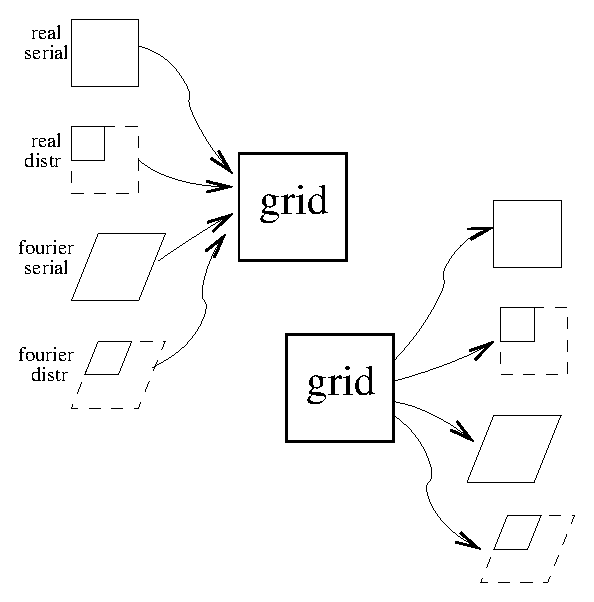
\epsfig{file=figs/grid.eps}
\caption{The grid type is used to glue together various field formats
as a general union operator}
\label{gridfig}
\end{center}
\end{figure}

The point of this section is to walk the reader through one Socorro
module and explain the general look and feel, so the reader can more
easily absorb the more complicated data types.  We use the source
\verb+grid_mod.f90+ from the date {Sep 26 16:03:21 MDT 2000},
with comments in the program text mostly stripped out, and lines
wrapped.

\begin{verbatim}
      module grid_mod

      use kind_mod
      use ghost_mod
      use core_mod
      use layout_mod

      private
\end{verbatim}
The grid module depends on only a few other modules.  Most notable of
these is the \verb+layout_mod+ which contains the primitive redistribution
and transformation functions that will be called from this module.  We
set the module private by default as in all Socorro modules to avoid
accidentally making internal functions public.

\begin{verbatim}
      type, public :: grid_obj
      private
      integer :: ref
      type(grid_ref), pointer :: o
      end type

      type grid_ref
      integer :: ref
      type(ghost) :: g
      integer :: type
      type(layout_obj) :: layout
      real(wpd), dimension(:,:,:), pointer :: rdata
      complex(wpd), dimension(:,:,:), pointer :: cdata
      end type 
\end{verbatim}
The internals of grid consist of a ghost field, a type field, a copy
of the layout to use in redistribution, and two data pointers.  The 
rep-invariant can be summarized by the following list of allowed states:
\begin{itemize}
\item type is \verb+EMPTY_KIND+: cdata is null, rdata is null
\item type is \verb+RS_KIND+   : cdata is null, rdata is serially dimensioned
\item type is \verb+RD_KIND+   : cdata is null, rdata is distributedly dimensioned
\item type is \verb+CSP_KIND+  : rdata is null, cdata is serially dimensioned
\item type is \verb+CDP_KIND+  : rdata is null, cdata is distributedly dimensioned
\item type is \verb+CSF_KIND+  : rdata is null, cdata is serially dimensioned
\item type is \verb+CDF_KIND+  : rdata is null, cdata is distributedly dimensioned
\end{itemize}
where ``dimensionalization is determined by the layout'' is equivalent to
the logical function \verb+consistent(\{rc\}data,layout,type)+ defined in
the module \verb+layout_mod+.

What then follows are the declarations of a whole bunch of 
overloaded functions.  The \verb+public+ declarations at the bottom
of this section summarize the public interface.
\begin{verbatim}
      interface grid
      module procedure grid_const
      end interface
      interface my
      module procedure my_grid, my_grid_new
      end interface
      interface thy
      module procedure thy_grid
      end interface
      interface bequeath
      module procedure bequeath_grid
      end interface
      interface glean
      module procedure glean_grid
      end interface
      interface take
      module procedure take_ptr_grid_r,take_ptr_grid_c
      end interface
      interface put
      module procedure put_ptr_grid_r,put_ptr_grid_c
      end interface
      interface x_type
      module procedure grid_type
      end interface
      interface x_layout
      module procedure grid_layout
      end interface
      interface x_ghost
      module procedure grid_ghost
      end interface
      interface assignment(=)
      module procedure assign_grid
      end interface

      public :: grid,my,thy,glean,bequeath,assignment(=)
      public :: x_type, x_layout, put, take
      public :: x_ghost
\end{verbatim}
Aside from the SADR functions, and functions to extract different
members of \verb+type(grid_obj)+, there are really two major functions
defined \verb+put+ which puts data on the grid and \verb+take+ which
takes data off the grid.

The garbage collection is just the simple lazy copied value method defined
in section \ref{lazysec}.  (Note: some of the private names for the overloaded
SADR procedures might vary from the examples in \ref{lazysec}.)

\begin{verbatim}
      subroutine my_grid_new(gi,G)
      type(grid_obj) ::gi,g
      g%ref = 1
      g%o => gi%o
      g%o%ref = g%o%ref+1
      end subroutine

      subroutine my_grid(G)
      type(grid_obj) g
      g%ref = g%ref+1
      g%o%ref = g%o%ref+1
      end subroutine

      function thy_grid(G) result(gout)
      type(grid_obj)::g,gout
      g%ref = g%ref-1
      g%o%ref = g%o%ref-1
      gout%ref = g%ref
      gout%o => g%o
      end function

      subroutine bequeath_grid(G)
      type(grid_obj) g
      continue
      end subroutine

      subroutine glean_grid(G)
      type(grid_obj) g
      if (g%o%ref<1) then
         select case (g%o%type)
         case (EMPTY_KIND)
            continue
         case (RD_KIND,RS_KIND)
            deallocate(g%o%rdata)
         case (CSP_KIND,CDP_KIND,CSF_KIND,CDF_KIND)
            deallocate(g%o%cdata)
         end select
         deallocate(g%o)
      end if
      end subroutine

      subroutine assign_grid(g1,g2)
      type(grid_obj), intent(inout) :: g1
      type(grid_obj), intent(in) :: g2
      type(grid_obj) gtmp
      call my(g2)
      if (error(x_ghost(g1%o%layout).ne.x_ghost(g2%o%layout), &
          "assigning grids of unequal layouts")) goto 100
      gtmp%o => g1%o
      g1%o%ref = g1%o%ref - g1%ref
      g1%o => g2%o
      g1%o%ref = g1%o%ref + g1%ref
      call glean(gtmp)
 100  call glean(thy(g2))
      end subroutine

\end{verbatim}

The grid constructor is defined by
\begin{verbatim}
      function grid_const(ly) result(g)
      type(grid_obj) g
      type(layout_obj), intent(in) :: ly
      g%ref = 0
      allocate(g%o)
      g%o%g = x_ghost()
      g%o%ref = 0
      g%o%type = EMPTY_KIND
      call my(ly,g%o%layout)
      nullify(g%o%rdata)
      nullify(g%o%cdata)
      end function
\end{verbatim}
which returns an empty grid to the caller.

\begin{verbatim}
      integer function grid_type(g)
      type(grid_obj), intent(in) :: g
      call my(g)
      grid_type = g%o%type
      call glean(thy(g))
      end function

      type(layout_obj) function grid_layout(g)
      type(grid_obj), intent(in) :: g
      call my(g)
      call my(g%o%layout,grid_layout)
      call bequeath(thy(grid_layout))
      call glean(thy(g))
      end function

      type(ghost) function grid_ghost(g)
      type(grid_obj), intent(in) :: g
      call my(g)
      grid_ghost = g%o%g
      call glean(thy(g))
      end function
\end{verbatim}
The functions above allow relevant information to be extracted
from grids like ghosts, the type of the currently stored
grid data, as well as the underlying layout of the grid itself
if needed.  All these functions have the property that they 
are cheap to call and do not have any side effects.
We got it into our heads to put an \verb+x_+ prefix in front of
such functions, and the convention generally stuck.

We can now move to those functions which mutate grid data.

\begin{verbatim}
      subroutine mutate_i(g)
      type(grid_obj) g
      type(grid_obj) gtmp
      if (g%ref < g%o%ref) then
         allocate(gtmp%o)
         gtmp%o%ref = 0
         call my(g%o%layout,gtmp%o%layout)
         gtmp%o%type = g%o%type
         select case (g%o%type)
         case (EMPTY_KIND)
            continue
         case (RD_KIND,RS_KIND)
            call alloc(gtmp%o%rdata,g%o%layout,g%o%type)
            gtmp%o%rdata = g%o%rdata
            nullify(gtmp%o%cdata)
         case (CSP_KIND,CDP_KIND,CSF_KIND,CDF_KIND)
            call alloc(gtmp%o%cdata,g%o%layout,g%o%type)
            gtmp%o%cdata = g%o%cdata
            nullify(gtmp%o%rdata)
         end select
         gtmp%o%g = g%o%g
         g%o%ref = g%o%ref - g%ref
         g%o => gtmp%o
         g%o%ref = g%o%ref + g%ref
      end if
      end subroutine
\end{verbatim}
In \verb+grid_mod+ the function for forking off a new grid is 
the private function \verb+mutate_i+.

\begin{verbatim}
      subroutine empty_grid_i(G)
      type(grid_obj), intent(inout) :: g
      select case (g%o%type)
      case (EMPTY_KIND)
         continue
      case (RD_KIND,RS_KIND)
         deallocate(g%o%rdata); nullify(g%o%rdata)
      case (CSP_KIND,CDP_KIND,CSF_KIND,CDF_KIND)
         deallocate(g%o%cdata); nullify(g%o%cdata)
      end select
      g%o%type = EMPTY_KIND
      end subroutine
\end{verbatim}
This is an internal utility to make sure a grid has no data on
it when new data is about to be put on it.  One notes that it
does not call \verb+mutate_i+ even though it modifies its argument,
but since it is a private procedure and is never called in a
context where forking is needed, that is ok.

\begin{verbatim}
      subroutine put_ptr_grid_r(DATA,G,kind)
      real(wpd), dimension(:,:,:), pointer :: data
      type(grid_obj), intent(inout) :: g
      integer, intent(in)    :: kind
      integer tpo
      real(wpd), dimension(:,:,:), pointer :: rtmp
      complex(wpd), dimension(:,:,:), pointer :: ctmp
      tpo = kind
      call my(g)
      call mutate_i(g)
      call empty_grid_i(g)
      if (error(.not.consistent(data,g%o%layout,kind), &
           "put_ptr_grid_r: inconsistent type for data")) goto 100
      rtmp => data;  nullify(ctmp);  nullify(data)
      call transfer_grid(g%o%layout,G%o%TYPE,G%o%RDATA,G%o%CDATA,  &
                         TPO,RTMP,CTMP)
      g%o%g = x_ghost()
 100  if (error("put_ptr_grid_r: ")) continue
      call glean(thy(g))
      end subroutine

      subroutine put_ptr_grid_c(DATA,G,kind)
      type(grid_obj), intent(inout) :: g
      integer, intent(in)    :: kind
      complex(wpd), dimension(:,:,:), pointer :: data
      integer  tpo
      real(wpd), dimension(:,:,:), pointer :: rtmp
      complex(wpd), dimension(:,:,:), pointer :: ctmp
      tpo = kind
      call my(g)
      call mutate_i(g)
      call empty_grid_i(g)
      if (error(.not.consistent(data,g%o%layout,kind), &
           "put_ptr_grid_c: inconsistent type for data")) goto 110
      ctmp => data;  nullify(rtmp);  nullify(data)
      call transfer_grid(g%o%layout,G%o%TYPE,G%o%RDATA,G%o%CDATA, &
                         TPO,RTMP,CTMP)
      g%o%g = x_ghost()
      if (error("put_ptr_grid_c: ")) continue
 110  call glean(thy(g))
      end subroutine
\end{verbatim}
The \verb+put_+ functions are nearly identical.  They fork \verb+g+,
then ensure that \verb+g+ is empty and that its layout is compatible with
the input data.  With that taken care of control is transferred to a 
hideous (private) pointer transformation function.

\begin{verbatim}
      subroutine take_ptr_grid_r(DATA,G,kind)
      real(wpd), dimension(:,:,:), pointer :: data
      type(grid_obj), intent(inout) :: g
      integer, intent(in)    :: kind
      integer tpo 
      real(wpd), dimension(:,:,:), pointer :: rtmp
      complex(wpd), dimension(:,:,:), pointer :: ctmp
      call my(g)
      call mutate_i(g)
      nullify(rtmp);  nullify(ctmp)
      tpo = kind
      call transfer_grid(g%o%layout,TPO,RTMP,CTMP,  &
                         G%o%TYPE,G%o%RDATA,G%o%CDATA)
      g%o%g = x_ghost()
      if (error("take_ptr_grid_r: ")) goto 120
      data => rtmp
      if (error(.not.consistent(data,g%o%layout,kind), &
          "take_ptr_grid_r: inconsistent type for data")) goto 120
 120  call glean(thy(g))
      end subroutine

      subroutine take_ptr_grid_c(DATA,G,kind)
      complex(wpd), dimension(:,:,:), pointer :: data
      type(grid_obj), intent(inout) :: g
      integer, intent(in)    :: kind
      integer  tpo
      real(wpd), dimension(:,:,:), pointer :: rtmp
      complex(wpd), dimension(:,:,:), pointer :: ctmp
      call my(g)
      call mutate_i(g)
      nullify(rtmp);  nullify(ctmp)
      tpo = kind
      call transfer_grid(g%o%layout,TPO,RTMP,CTMP,  &
                         G%o%TYPE,G%o%RDATA,G%o%CDATA)
      g%o%g = x_ghost()
      if (error("take_ptr_grid_c: ")) goto 130
      data => ctmp
      if (error(.not.consistent(data,g%o%layout,kind), &
          "take_ptr_grid_c: inconsistent type for data")) goto 130
 130  call glean(thy(g))
      end subroutine
\end{verbatim}
Take is much the same.  A fork, followed by some checks, followed by
the hideous pointer transformation function.

The pointer transformation function which is essentially wrapped
by \verb+put+ and \verb+take+ procedures simply calls the right
layout transformations to get the data from one form to another.
Although it is not public, it is of sufficient complexity that the author
felt it deserved some commentary specification in order to keep it 
organized and maintainable.

\begin{verbatim}
      recursive subroutine transfer_grid(ly,OTYPE,ORDATA,OCDATA, &
          ITYPE,IRDATA,ICDATA)
      type(layout_obj), intent(in) :: ly
      integer  :: otype, itype
      real(wpd),dimension(:,:,:), pointer :: ordata,irdata,rtmp
      complex(wpd),dimension(:,:,:), pointer :: ocdata,icdata,ctmp
      integer, dimension(3) :: dims, locdims
! This routine needs some elaboration, even though it is private and internal
! requires: otype,ordata,ocdata be consistent with the fields of a grid type
!           itype,irdata,icdata be consistent with the fields of a grid type
! errors: if otype is empty, but passes errors
! modifies: otype,ordata,ocdata,itype,irdata,icdata
! performs the pointer swap, and conversion required to transfer the 
! idata to the odata.
! for debugging the recursion
!      write(iobuf,*) "call to transfer ",otype,itype; call warn(iobuf)
      call my(ly)
      if(error(itype.eq.EMPTY_KIND,"grid_mod: empty data source")) return 
      dims = x_dims(ly)
      locdims = x_locdims(ly)
      if (otype.eq.EMPTY_KIND.or.otype.eq.itype) then
! (base case) transfer all data for empty or equal types
         otype = itype; itype = EMPTY_KIND
         ordata => irdata; nullify(irdata)
         ocdata => icdata; nullify(icdata)
         return
! going from complex to real has highest priority 1
      elseif (itype.eq.CSP_KIND.and. &
              (otype.eq.RS_KIND.or.otype.eq.RD_KIND)) then
         itype = RS_KIND
         call alloc(irdata,ly,itype)
         irdata = real(icdata,KIND=wpd)
         deallocate(icdata)
      elseif (itype.eq.CDP_KIND.and.  &
              (otype.eq.RS_KIND.or.otype.eq.RD_KIND)) then
         itype = RD_KIND
         call alloc(irdata,ly,itype)
         irdata = real(icdata,KIND=wpd)
         deallocate(icdata)
! if a scatter is necessary then it should be done with priority 2
      elseif ( (itype.eq.RS_KIND).AND.  &
               ((otype.eq.RD_KIND).or.  &
                (otype.eq.CDP_KIND).or.  &
                (otype.eq.CDF_KIND) )  ) then
         rtmp => irdata
         itype = RD_KIND
         call alloc(irdata,ly,itype)
         call warn("grid_mod: doing scatter")
         call scatter(ly,rtmp,IRDATA)
         deallocate(rtmp)
      elseif ( ((itype.eq.CSP_KIND).or.  &
                (itype.eq.CSF_KIND) ).AND.  &
               ((otype.eq.RD_KIND).or.  &
                (otype.eq.CDP_KIND).or.  &
                (otype.eq.CDF_KIND) )  ) then
         ctmp => icdata
         if (itype==CSP_KIND) itype = CDP_KIND
         if (itype==CSF_KIND) itype = CDF_KIND
         call alloc(icdata,ly,itype)
         call warn("grid_mod: doing scatter")
         call scatter(ly,ctmp,ICDATA)
         deallocate(ctmp)
! complexification and fourier transformation are of equal priority 3
      elseif ( itype.eq.RS_KIND  .AND.  &
               (otype.eq.CSP_KIND.or.  &
                otype.eq.CSF_KIND ) ) then
               itype = CSP_KIND
               call alloc(icdata,ly,CSP_KIND)
               icdata = cmplx(irdata,KIND=wpd)
               deallocate(irdata)
      elseif ( itype.eq.RD_KIND  .AND.  &
               (otype.eq.CSP_KIND.or.  &
                otype.eq.CSF_KIND.or.  &
                otype.eq.CDP_KIND.or.  &
                otype.eq.CDF_KIND ) ) then
         itype = CDP_KIND
         call alloc(icdata,ly,itype)
         icdata = cmplx(irdata,0.0d0)
         deallocate(irdata)
      elseif ( (itype.eq.CSP_KIND).AND.(otype.eq.CSF_KIND) ) then
         call fft_serial(ly,icdata,r_to_q); itype=CSF_KIND
      elseif ( (itype.eq.CSF_KIND).AND.  &
              (otype.eq.CSP_KIND.or.otype.eq.RS_KIND) ) then
         call fft_serial(ly,icdata,q_to_r); itype=CSP_KIND
      elseif ( (itype.eq.CDP_KIND).AND.  &
                (otype.eq.CSF_KIND.or.otype.eq.CDF_KIND) ) then
         call warn("grid_mod: doing parallel fft")
         call fft_parallel(ly,icdata,r_to_q); itype=CDF_KIND
      elseif ( (itype.eq.CDF_KIND).AND.  &
                (otype.eq.CSP_KIND.or.otype.eq.CDP_KIND.or.  &
                otype.eq.RS_KIND.or.otype.eq.RD_KIND) ) then
         call warn("grid_mod: doing parallel fft")
         call fft_parallel(ly,icdata,q_to_r); itype=CDP_KIND
! gather steps are performed with lowest priority 4
      elseif ( (itype.eq.RD_KIND).AND.(otype.eq.RS_KIND)) then
         itype = RS_KIND
         rtmp => irdata; 
         call alloc(irdata,ly,itype)
         call warn("grid_mod: doing gather")
         call gather(ly,rtmp,irdata)
         deallocate(rtmp)
      elseif ( (itype.eq.CDP_KIND.or.itype.eq.CDF_KIND)  &
              .AND.(otype.eq.CSP_KIND.or.otype.eq.CSF_KIND)) then
         if (itype.eq.CDP_KIND) itype = CSP_KIND
         if (itype.eq.CDF_KIND) itype = CSF_KIND
         ctmp => icdata
         call alloc(icdata,ly,itype)
         call warn("grid_mod: doing gather")
         call gather(ly,ctmp,icdata)
         deallocate(ctmp)
      end if
! we should now have moved one step towards termination, so we call again
      if (error("grid_mod : ")) return
      call transfer_grid(ly,OTYPE,ORDATA,OCDATA,  &
           ITYPE,IRDATA,ICDATA)
      call glean(thy(ly))
      end subroutine

      end module grid_mod
\end{verbatim}




